\subsection{The Lagrangian Method: Mechanics Without Diagrams}

\textbf{What if you could describe the motion of the planets — not with diagrams or forces — but with a single elegant equation?}

That’s exactly what Joseph-Louis Lagrange set out to do.

He didn’t begin as a traditional academic. In fact, Lagrange was almost entirely self-taught. Born in Turin, he discovered mathematics not through formal education, but through fascination — especially with the emerging power of calculus. His genius revealed itself early, and as a teenager, he began corresponding with one of the most dominant scientific minds of the century: \textbf{Leonhard Euler}.

What began as letters turned into a mentorship. Euler quickly recognized Lagrange’s brilliance and supported his ascent into the heart of European science. But Lagrange didn’t just follow in Euler’s footsteps — he reimagined the very foundations of mechanics.

While Newton's vision of physics was geometric and visually intuitive, Lagrange aimed to rewrite it as pure algebra. No diagrams, no triangles, no intuitive pushes or pulls. Just symbols. He wanted to understand how systems moved not by drawing them, but by asking what paths nature would prefer — and why.

This ambition wasn’t just mathematical — it was deeply philosophical. Lagrange lived in the heart of the Enlightenment, a period obsessed with reason, structure, and determinism. The thinkers of his age believed the universe operated like a rational machine: every part in lawful relation to every other, governed by principles that, if known, could explain everything:  ``Give me the initial conditions,'' said Laplace, ``and I will predict the future.''

This idea—that nature was fully intelligible, fully lawful, and fully determined—was the philosophical air Lagrange breathed. Newton had already shown that the planets moved by universal laws. But Newton’s mechanics still relied on force—something that required visualization, contact, sometimes even intuition.

Lagrange wanted something cleaner. Something inevitable.

He was after a language of motion where \textbf{everything followed from first principles}, not as a story of objects bumping into each other, but as a logic of preference — as if nature were solving a symbolic optimization problem at every moment.

The result was revolutionary: a new formalism built not on forces, but on \textbf{energy} and \textbf{efficiency}. This framework culminated in what we now call the \textbf{principle of least action}.

\begin{quote}
    Instead of tracking how forces push on particles, Lagrange asked: out of all possible ways a system could move from one configuration to another, which path does nature actually choose?
\end{quote}

\begin{figure}[H]
    \centering
    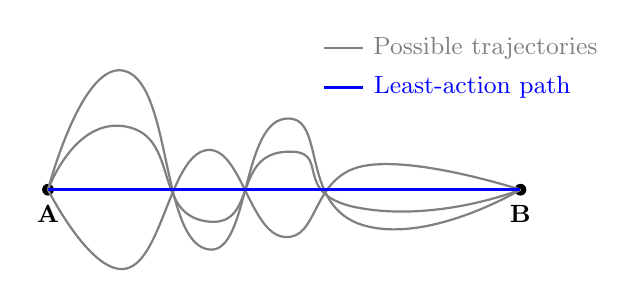
\begin{tikzpicture}[scale=1, every node/.style={font=\small}]
      % Points A and B
      \node[fill=black, circle, inner sep=1.5pt, label=below:{\textbf{A}}] (A) at (0,0) {};
      \node[fill=black, circle, inner sep=1.5pt, label=below:{\textbf{B}}] (B) at (6,0) {};
  
      % Legend
      \begin{scope}[shift={(3.5,1.8)}]
        \draw[gray, thick] (0,0) -- (0.5,0) node[right, font=\small]{Possible trajectories};
        \draw[blue, very thick] (0,-0.5) -- (0.5,-0.5) node[right, font=\small]{Least‐action path};
      \end{scope}
  
      % Multiple possible paths (gray)
      \foreach \yshift/\tension in {1.5/1, -1/0.8, 0.8/1.2} {
        \draw[gray, thick]
          plot [smooth, tension=\tension]
          coordinates {(A) (1,\yshift) (2,-0.5*\yshift) (3,0.6*\yshift) (4,-0.3*\yshift) (B)};
      }
  
      % Chosen least-action path (blue & thicker)
      \draw[blue, very thick]
        plot [smooth, tension=1]
        %coordinates {(A) (1,0.8) (2,0.3) (3,-0.1) (4,0.2) (B)}
        coordinates {(A) (B)}
        node[pos=0.5, above, sloped] {};
    \end{tikzpicture}
    \caption{Several possible paths from point A to B (gray) with the path of least action highlighted (blue).}
\end{figure}
  
  


